%!TEX root=presentation.tex
\section*{}

\begin{frame}
	\frametitle{Replication based matrix multiplication}
	\begin{center}
	\includegraphics[width=\textwidth]{images/rmm.png}
	\end{center}
\end{frame}	

\begin{frame}
	\frametitle{Cross product based matrix multiplication}
	\begin{center}
	\includegraphics[height=0.8\textheight]{images/cpmm.png}
	\end{center}
\end{frame}

\begin{frame}
	\frametitle{Communication costs}
	\begin{itemize}
		\item Matrix $A$ blocked with $M \times K$ blocks and $B$ blocked with $K \times N$ blocks
		\item Network and IO costs are dominant
		\item $costs_{RMM} \in O\left(network(|A|\cdot N + |B|\cdot M) + io(|A|+|B|+|C|)\right)$
		\item $costs_{CPMM} \in O\left(network(|A|+|B|+r\cdot|C|) + io(|A|+|B|+|C|) \right)$ with $r$ being the number of reducer
	\end{itemize}
\end{frame}

\begin{frame}
	\frametitle{Stratosphere execution plan}
	\begin{columns}
		\begin{column}{0.5\textwidth}
			\begin{itemize}
				\item Assuming row-wise partitioning of matrix $A$
				\item Execution plans for RMM and CPMM identical
				\item Differ only in chosen strategy for join operator
				\item RMM: Hybrid-hash join
				\item CPMM: Sort-merge join
				\item Stratosphere's optimizer chooses right plan
			\end{itemize}
		\end{column}
		\begin{column}{0.5\textwidth}
			\includegraphics[width=0.9\textwidth]{images/matrixMult.png}
		\end{column}
	\end{columns}
\end{frame}